\chapter{Design and Analysis} \label{Design and Analysis}
\section{Main Frame} \label{Main Frame 1}
The frame is designed to bear a total weight of 65 kg. The materials taken into consideration were Steel, Aluminium and Stainless Steel based on material selection criteria’s such as performance requirements, material reliability, safety, physical attributes, environmental conditions, availability, disposability, recyclability and economic factors.
The material required had to be corrosion resistant, light weight and economic.
Simulation for all three materials were carried out and stainless steel was selected.
\begin{table}[!ht]
\resizebox{\columnwidth}{!}{%
\begin{tabular}{|c|c|c|c|c|c|c|c|c|c|} 
\hline
\multicolumn{10}{|c|}{Main Frame}                                                                                             \\ 
\hline
Material        & \multicolumn{3}{c|}{Safety Factor} & \multicolumn{3}{c|}{Stress (MPa)} & \multicolumn{3}{c|}{Displacement}  \\ 
\hline
                & Threshold & Min  & Max             & Threshold & Min & Max             & Threshold & Min & Max              \\ 
\hline
Steel           & 0-8       & 4.35 & 15              & 0-47.59   & 0   & 47.59           & 0-0.7278  & 0   & 0.7278           \\ 
\hline
Aluminium       & 0-8       & 5.8  & 15              & 0-47.38   & 0   & 47.38           & 0-2.216   & 0   & 2.216            \\ 
\hline
Stainless Steel & 0-8       & 5.25 & 15              & 0-47.49   & 0   & 47.49           & 0-0.7919  & 0   & 0.7919           \\
\hline
\end{tabular}%
}
\caption{Stress and Displacement Analysis of Main Frame}
\end{table}




\begin{figure}[H]
\subfigure[Main Frame Safety Factor]
	{
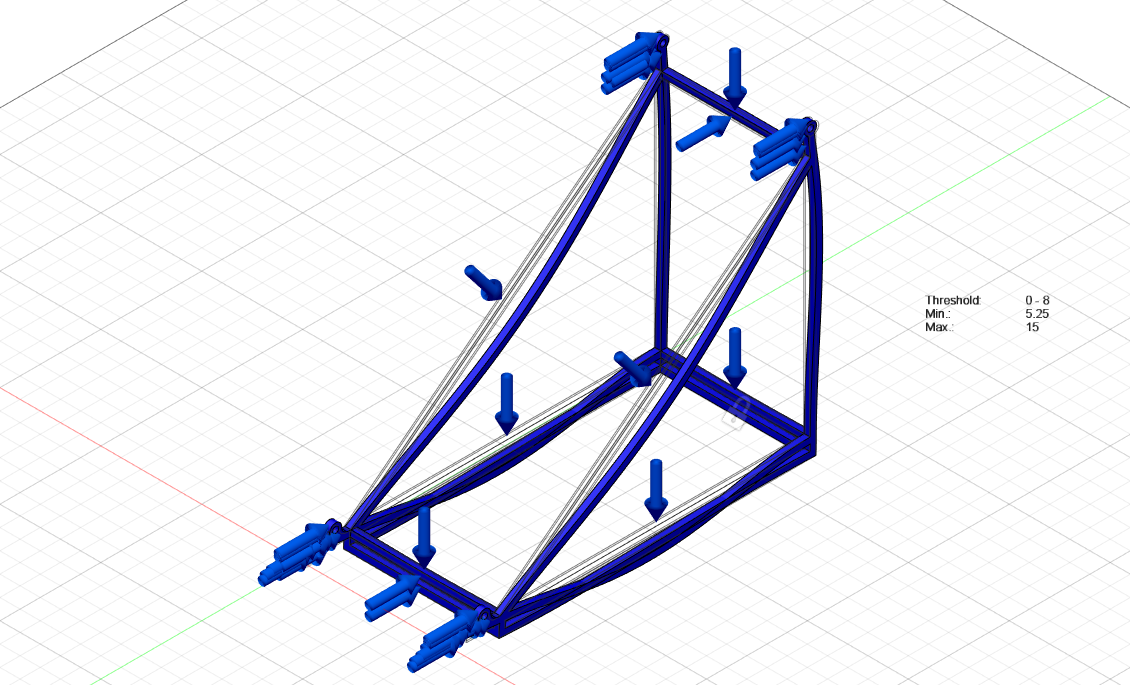
\includegraphics[scale=0.2]{MainFrameFOS}
\label{fig:a1}
	}
\subfigure[Main Frame Stress Distribution]
	{
	\label{fig:b1}
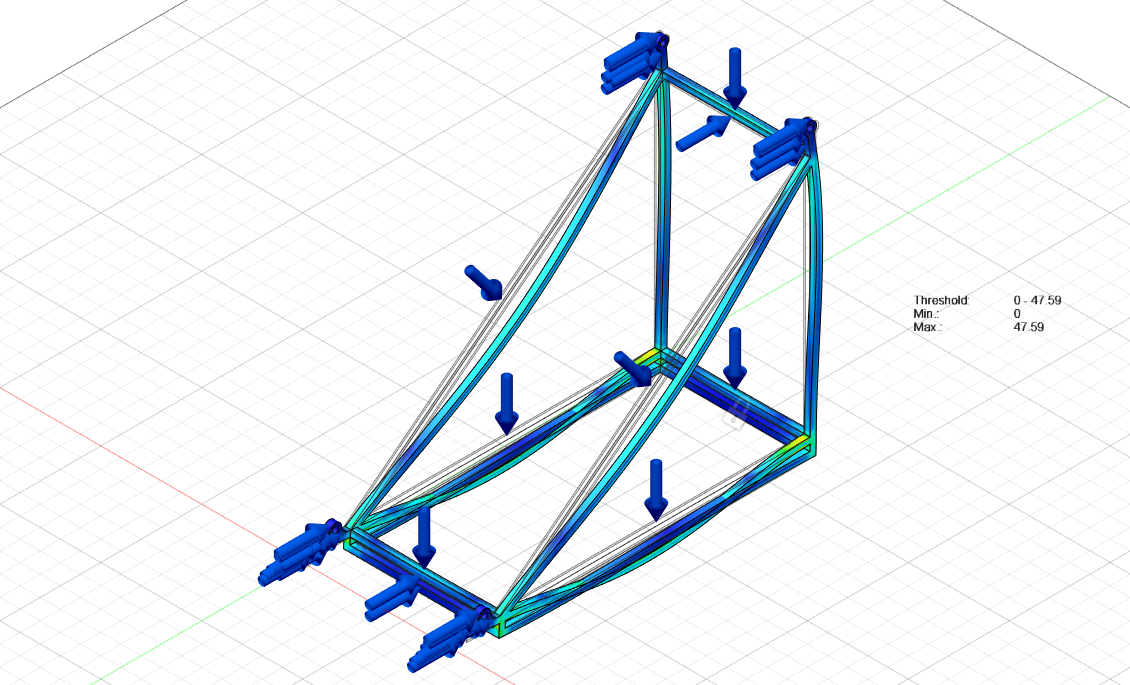
\includegraphics[scale=0.2]{MainFrameStress}
	}
\subfigure[Main Frame Displacement]
	{
	\label{fig:c1}
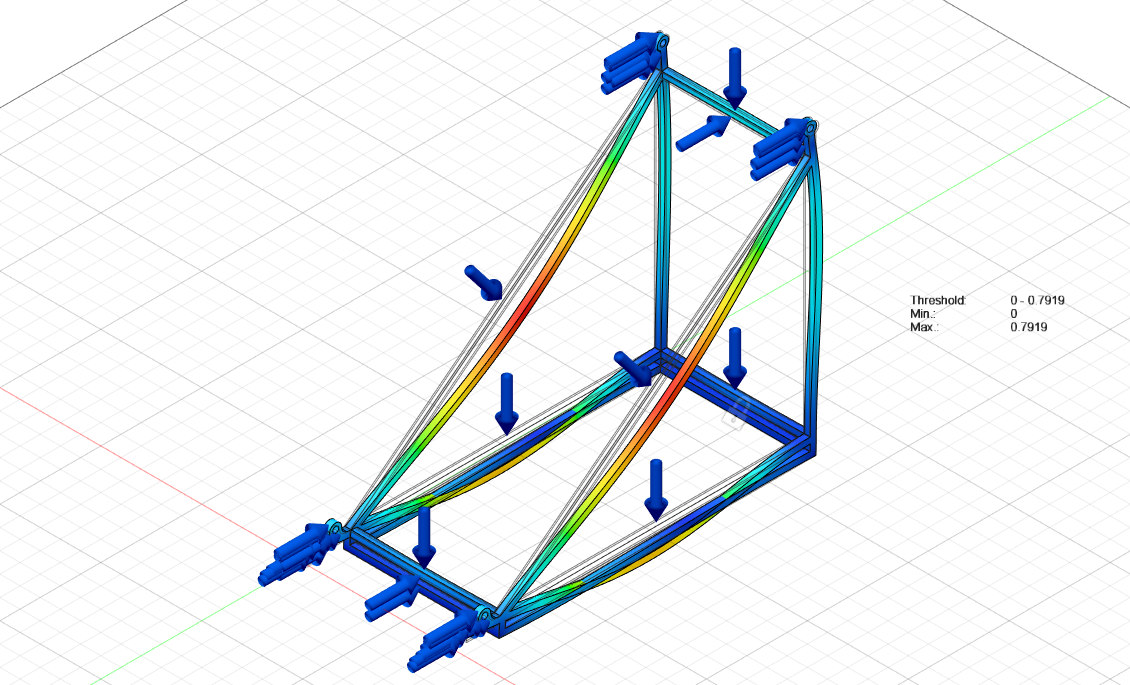
\includegraphics[scale=0.2]{Mainframedisplacement}
	}
\caption{Main Frame simulation analysis}

\end{figure}






\section{Front Scraper} \label{Front Scraper 1}
The front scraper is designed to scrape off cow dung from the ground and push it over to the bottom plate. The scraper must be sturdy enough that it can sustain prolonged shear stress due to friction and flexible enough that it can be forced to be as close to the ground as possible without premature plastic deformation. Flexible PVC material is chosen for its durability and flexibility, and it's low weight. Stainless steel also was analysed, the results are shown in the table.
\begin{table}[!ht]
\resizebox{\columnwidth}{!}{%
\begin{tabular}{|c|c|c|c|c|c|c|c|c|c|} 
\hline
\multicolumn{10}{|c|}{Front Scraper}                                                                                          \\ 
\hline
Material        & \multicolumn{3}{c|}{Safety Factor} & \multicolumn{3}{c|}{Stress (MPa)} & \multicolumn{3}{c|}{Displacement}  \\ 
\hline
                & Threshold & Min & Max              & Threshold & Min & Max             & Threshold & Min & Max              \\ 
\hline
PVC Flexible    & 0-8       & 15  & 15               & 0-0.2106  & 0   & 0.2106          & 0-115.3   & 0   & 115.3            \\ 
\hline
Stainless Steel & 0-8       & 15  & 15               & 0-0.2186  & 0   & 0.2186          & 0-0.0044  & 0   & 0.0044           \\
\hline
\end{tabular}%
}
\caption{Stress and Displacement Analysis of Front Scraper}
\end{table}

\begin{figure}[H]
\subfigure[Front Scraper Safety Factor]
	{
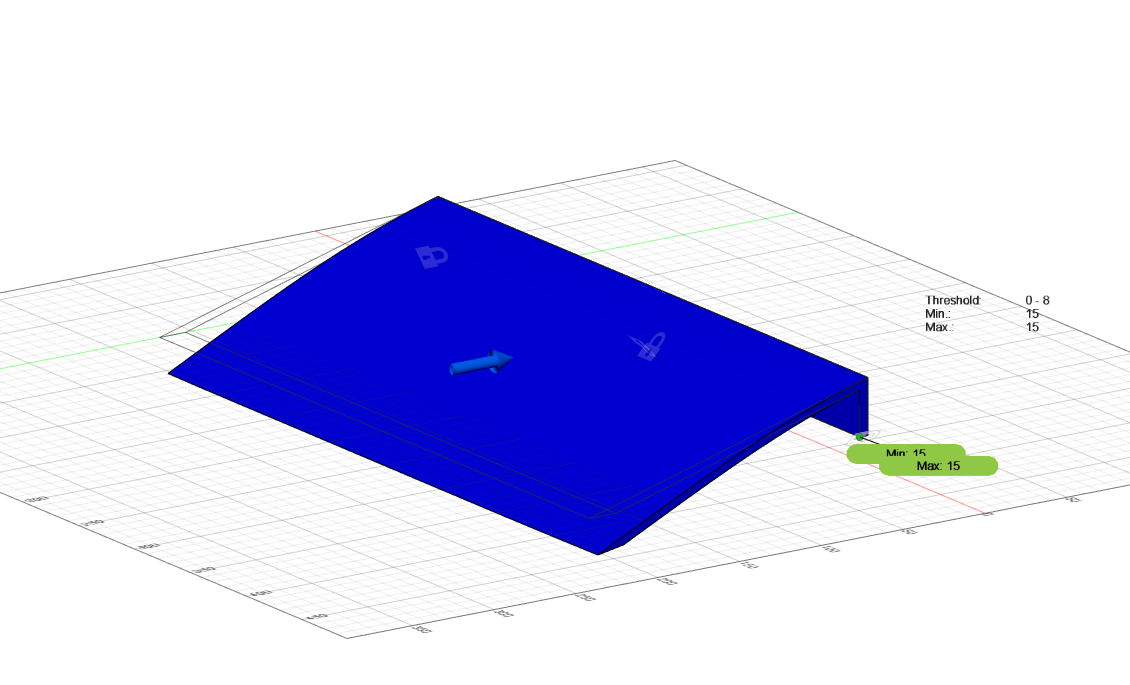
\includegraphics[scale=0.2]{FrontscraperFOS}
\label{fig:a2}
	}
\subfigure[Front Scraper Stress Distribution]
	{
	\label{fig:b2}
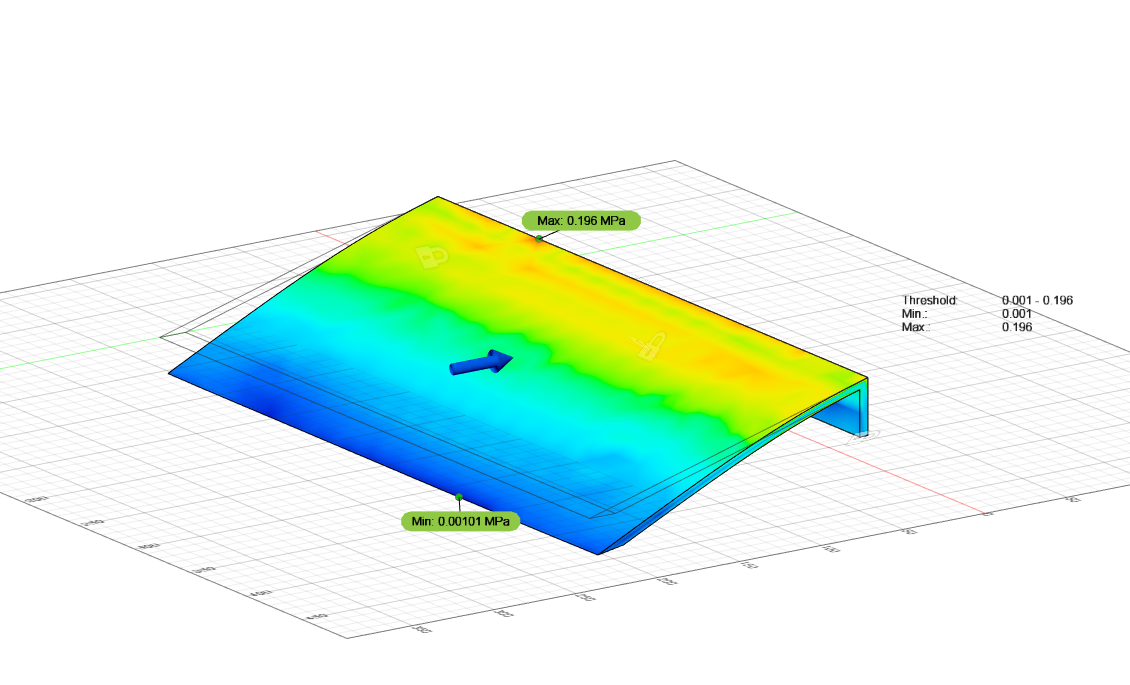
\includegraphics[scale=0.2]{FrontscraperStress}
	}
\subfigure[Front Scraper Displacement]
	{
	\label{fig:c2}
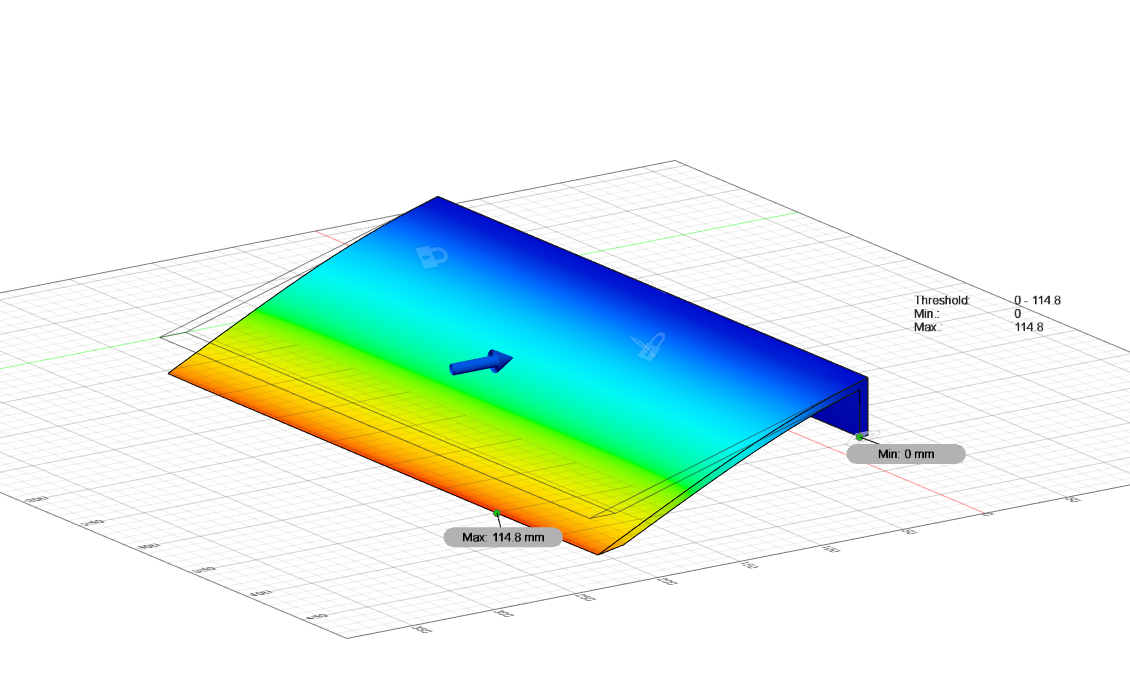
\includegraphics[scale=0.2]{FrontscraperDisplacement}
	}
\caption{Front Scraper simulation analysis}

\end{figure}
 


\section{Bottom Plate} \label{Bottom Plate 1}
Bottom Plate for the cow dung to be slid onwards to the storage bin. It must be designed to withstand normal stress due to the weight of cow dung and shear stress due to the friction between cow dung and the plates surface when it's being pushed onwards into the storage bin. The bottom plate must have high corrosive resistance. Stainless Steel is preferred material to fabricate this plate due to it's high corrosion resistance. Aluminum is also analysed but not preferred due to its high cost.


\begin{table}[!ht]
\resizebox{\columnwidth}{!}{%
\begin{tabular}{|c|c|c|c|c|c|c|c|c|c|} 
\hline
\multicolumn{10}{|c|}{Bottom Plate for Mount}                                                                                 \\ 
\hline
Material        & \multicolumn{3}{c|}{Safety Factor} & \multicolumn{3}{c|}{Stress (MPa)} & \multicolumn{3}{c|}{Displacement}  \\ 
\hline
                & Threshold & Min  & Max             & Threshold & Min & Max             & Threshold & Min & Max              \\ 
\hline
Stainless Steel & 0-8       & 2.76 & 15              & 0-90.6    & 0   & 90.6            & 0-4.687   & 0   & 4.687            \\ 
\hline
Aluminium       & 0-8       & 3.11 & 15              & 0-88.4    & 0   & 88.4            & 0-12.81   & 0   & 12.81            \\
\hline
\end{tabular}%
}
\caption{Stress and Displacement analysis of Bottom Plate}
\end{table}

\begin{figure}[H]
\subfigure[Bottom plate Safety Factor]
	{
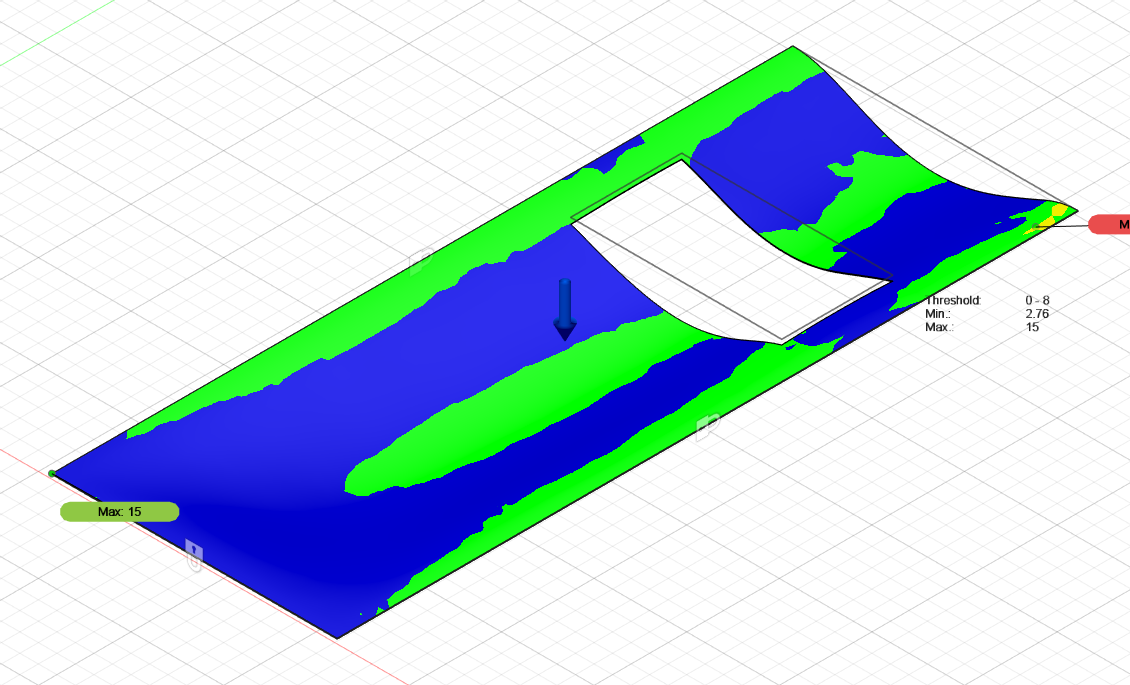
\includegraphics[scale=0.2]{BottomplateformountFOS}
\label{fig:a3}
	}
\subfigure[Bottom Plate Stress Distribution]
	{
	\label{fig:b3}
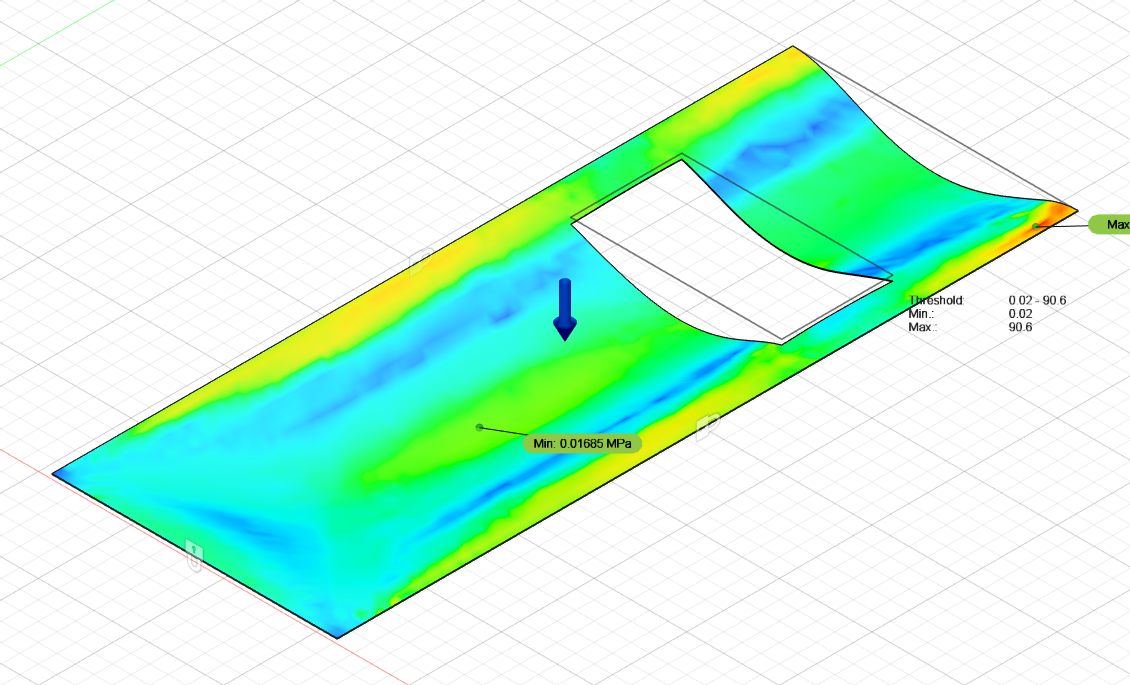
\includegraphics[scale=0.2]{BottomplateformountStress}
	}
\subfigure[Bottom Plate Displacement]
	{
	\label{fig:c3}
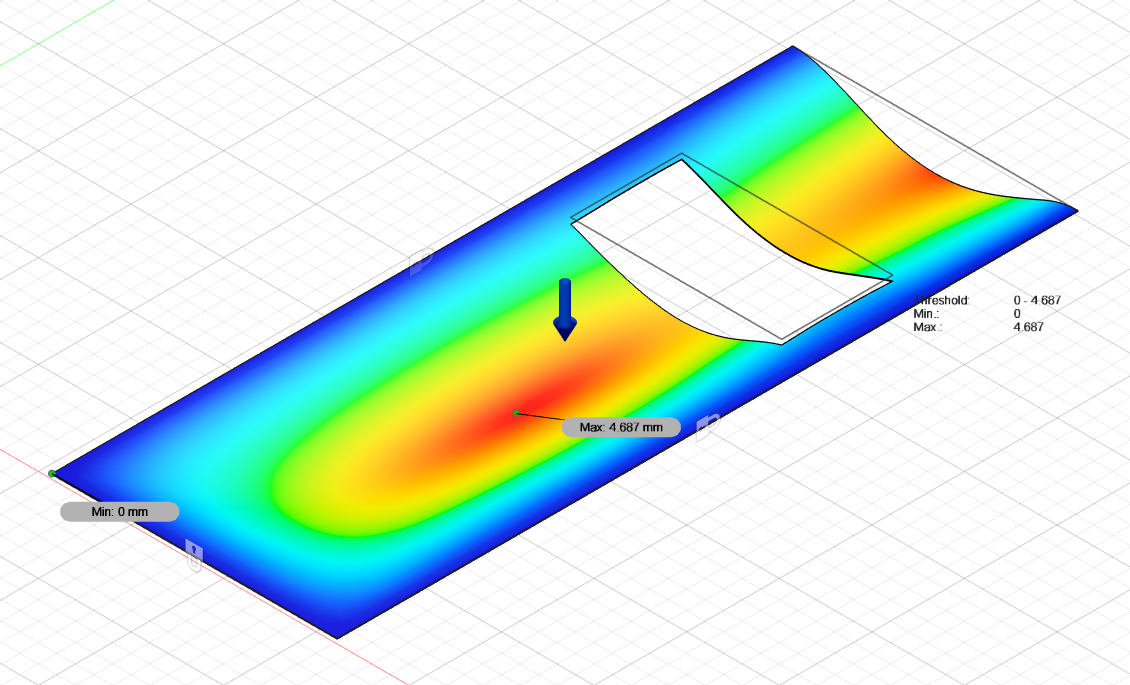
\includegraphics[scale=0.2]{BottommountDisplacement}
	}
\caption{Bottom Mount simulation analysis}

\end{figure}
 



\section{Blades Assembly} \label{Blades and Mount Assembly}
The blades do the job of collecting the cow dung from the front scraper and dumping it in the storage compartment. For this the materials which were taken into consideration for the design of the blades, which would be placed on a mount on the cow dung collector were Steel, Rubber Silicone and Flexible PVC, which were chosen based on the material selection criteria that we had decided. \\

Out of these materials, on performing simulation we found that having the blades made out of Steel would be most suitable for our mechanism to be efficient, and long lasting. \\

\begin{table}[!ht]
\resizebox{\columnwidth}{!}{%
\begin{tabular}{|cccccccccc|}
\hline
\multicolumn{10}{|c|}{Blades Assembly}                                                                                                                                                                                                                                                        \\ \hline
\multicolumn{1}{|c|}{Material}        & \multicolumn{3}{c|}{Safety Factor}                                                    & \multicolumn{3}{c|}{Stress (MPa)}                                                      & \multicolumn{3}{c|}{Displacement}                                  \\ \hline
\multicolumn{1}{|c|}{}                & \multicolumn{1}{c|}{Threshold} & \multicolumn{1}{c|}{Min}  & \multicolumn{1}{c|}{Max} & \multicolumn{1}{c|}{Threshold} & \multicolumn{1}{c|}{Min} & \multicolumn{1}{c|}{Max}   & \multicolumn{1}{c|}{Threshold} & \multicolumn{1}{c|}{Min} & Max    \\ \hline
\multicolumn{1}{|c|}{Steel}           & \multicolumn{1}{c|}{0-8}       & \multicolumn{1}{c|}{15}   & \multicolumn{1}{c|}{15}  & \multicolumn{1}{c|}{0-12.41}   & \multicolumn{1}{c|}{0}   & \multicolumn{1}{c|}{12.41} & \multicolumn{1}{c|}{0-0.0608}  & \multicolumn{1}{c|}{0}   & 0.0608 \\ \hline
\multicolumn{1}{|c|}{Rubber Silicone} & \multicolumn{1}{c|}{0-8}       & \multicolumn{1}{c|}{0.39} & \multicolumn{1}{c|}{15}  & \multicolumn{1}{c|}{0-534.4}   & \multicolumn{1}{c|}{0}   & \multicolumn{1}{c|}{534.4} & \multicolumn{1}{c|}{0-2340}    & \multicolumn{1}{c|}{0}   & 2340   \\ \hline
\multicolumn{1}{|c|}{PVC Flexible}    & \multicolumn{1}{c|}{0-8}       & \multicolumn{1}{c|}{1.33} & \multicolumn{1}{c|}{15}  & \multicolumn{1}{c|}{0-155.8}   & \multicolumn{1}{c|}{0}   & \multicolumn{1}{c|}{155.8} & \multicolumn{1}{c|}{0-1296}    & \multicolumn{1}{c|}{0}   & 1296   \\ \hline
\end{tabular}%
}
\caption{Stress and Displacement Analysis of Blades Assembly}
\end{table}


\begin{figure}[H]
\subfigure[Blades Assembly Safety Factor]
	{
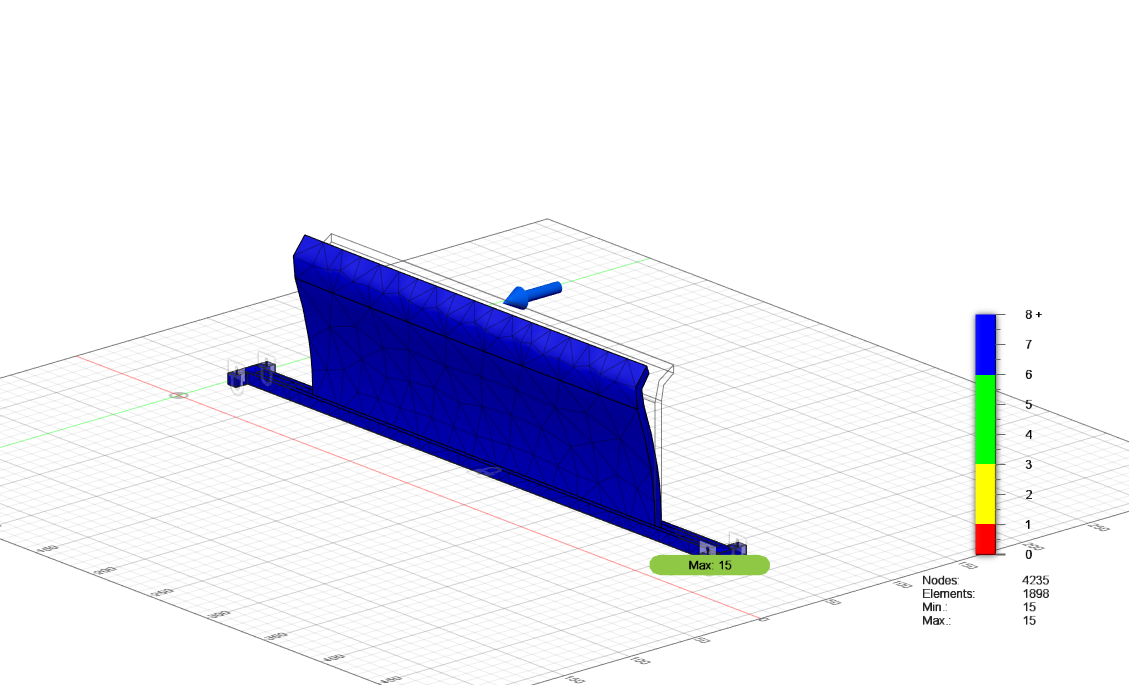
\includegraphics[scale=0.2]{BladeonMountFOS}
\label{fig:a4}
	}
\subfigure[Blades Assembly Stress Distribution]
	{
	\label{fig:b4}
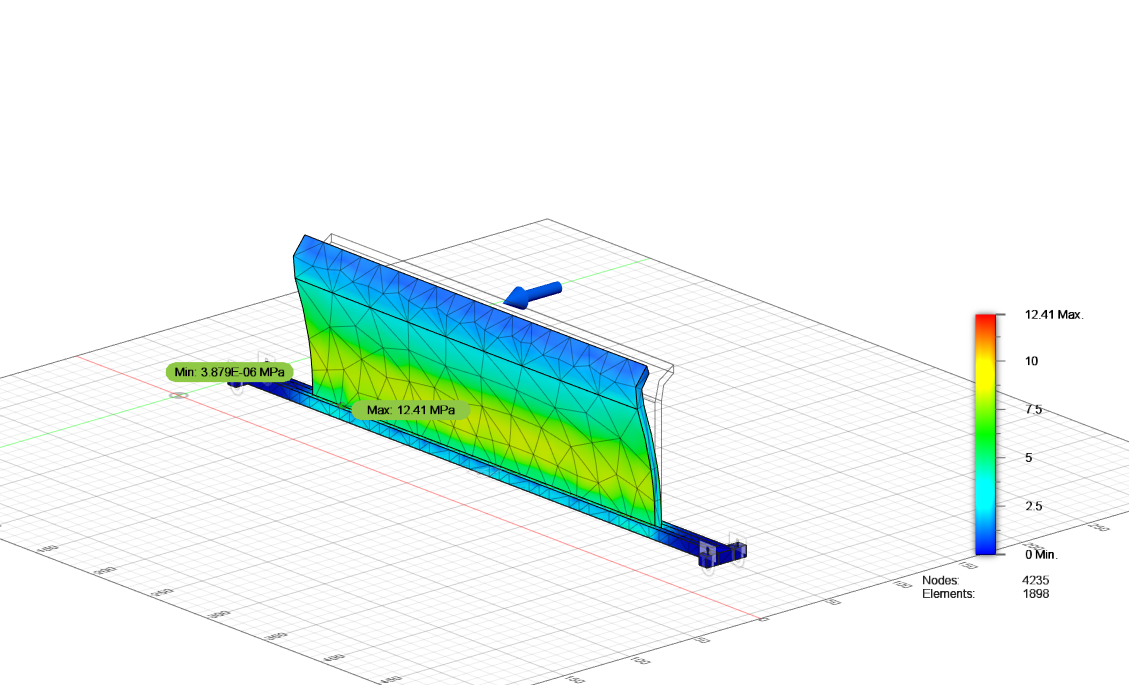
\includegraphics[scale=0.2]{BladeonMountStress}
	}
\subfigure[Blades Assembly Displacement]
	{
	\label{fig:c4}
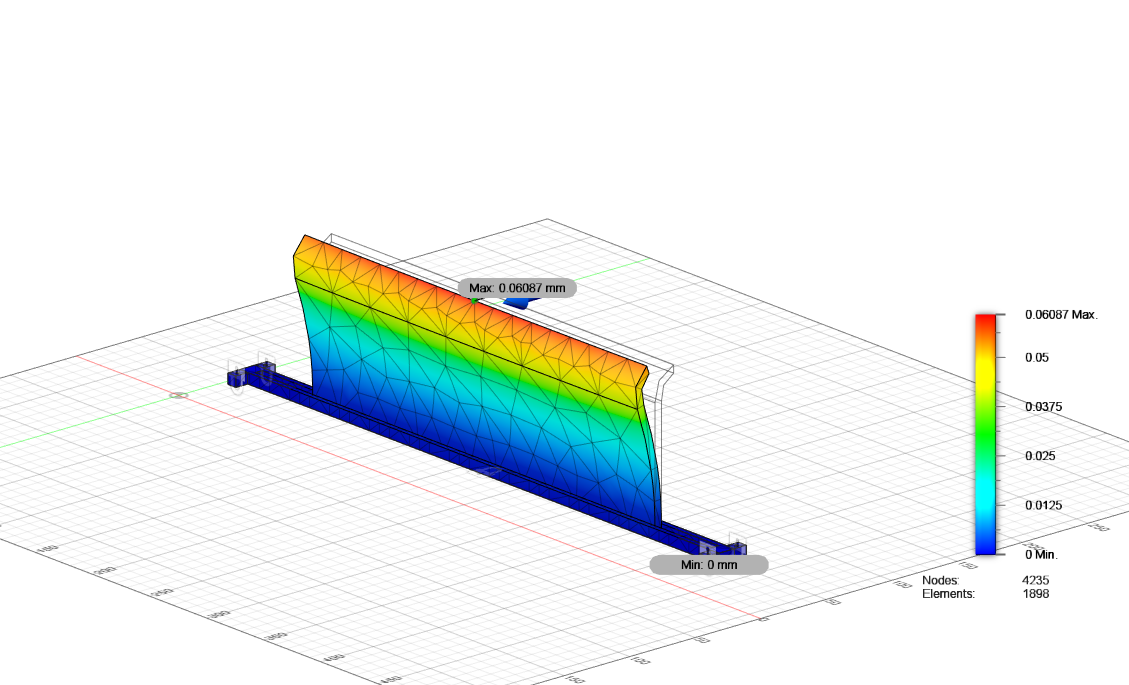
\includegraphics[scale=0.2]{BladeonMountDisplacement}
	}
\caption{Blades Assembly simulation analysis}

\end{figure}
